\documentclass[11pt]{beamer}
\usepackage{booktabs,siunitx}
\usepackage[default]{opensans}
\usetheme{Madrid}
\usefonttheme{default}
\useinnertheme{circles}
\sisetup{detect-all}
\setbeamertemplate{navigation symbols}{} % Uncomment this line to remove the navigation symbols from the bottom of all slides

\title[ALICE Run 3 Look-see]{``Look-see'' at pilot beam data for Run 3 at ALICE} % The short title in the optional parameter appears at the bottom of every slide, the full title in the main parameter is only on the title page

% \subtitle{Optional Subtitle} % Presentation subtitle, remove this command if a subtitle isn't required

\author[Miles Kidson]{Miles Kidson \\[1ex] {\small Supervisors: Prof. Zinhle Buthelezi \and Dr. SV Fortsch \and Prof. Tom Dietel \\ Assisted By Dr. B Naik (Postdoctoral fellow)}} % Presenter name(s), the optional parameter can contain a shortened version to appear on the bottom of every slide, while the main parameter will appear on the title slide

\institute[UCT]{University of Cape Town \\ \smallskip \textit{kdsmil001@myuct.ac.za}} % Your institution, the optional parameter can be used for the institution shorthand and will appear on the bottom of every slide after author names, while the required parameter is used on the title slide and can include your email address or additional information on separate lines

\date[September 2022]{Honour's Research Project \\ 2022} % Presentation date or conference/meeting name, the optional parameter can contain a shortened version to appear on the bottom of every slide, while the required parameter value is output to the title slide

\titlegraphic{\includegraphics[width=35pt]{Figs/ALICE_logo.png}}
\logo{\includegraphics[width=20pt]{Figs/ALICE_logo_transparent.png}}

\useoutertheme[subsection=false]{miniframes}

\begin{document}

\frame[plain]{\titlepage}

\section{Background}

\begin{frame}
    \frametitle{ALICE Run 3}

    \begin{columns}[c]
        \begin{column}{0.5\textwidth}
            \begin{figure}[h]
                \begin{center}
                    \includegraphics[width=\textwidth]{Figs/ALICE_RUN3_schematic_cropped.png}
                \end{center}
            \end{figure}
        \end{column}

        \begin{column}{0.5\textwidth}
            \begin{itemize}
                \item LHC Run 3 aims to increase $\sqrt{s}$ and luminosity of collisions
                \item At ALICE, the MFT (9) was added and ITS (6, 7) was upgraded
                \item Readout electronics for many detectors were also upgraded
                \item To manage Run 3 and ALICE's new untriggered data capture, the analysis framework was overhauled entirely
            \end{itemize}
        \end{column}
    \end{columns}

\end{frame}


\begin{frame}
    \frametitle{Coordinate System}

    \begin{columns}[t]
        \begin{column}{0.6\textwidth}
            \begin{itemize}
                \item $Z$: Distance along $Z$-axis (\unit{\centi\metre})
                \item $\varphi$: Azimuthal angle around beam axis
                \item $\theta$: Polar angle
            \end{itemize}
            \begin{figure}[h]
                \begin{center}
                    \includegraphics[width=\textwidth]{Figs/coords.pdf}
                \end{center}
            \end{figure}
        \end{column}

        \begin{column}{0.4\textwidth}
            \begin{itemize}
                \item $p_{\mathrm{T}}$: Transverse momentum (\unit{\giga\electronvolt\per c})
                \begin{equation*}
                    p_{\mathrm{T}}=\sqrt{p_x^2+p_y^2}
                \end{equation*}
                \item $y$: Rapidity
                \begin{equation*}
                    y=\frac{1}{2}\ln \frac{E+p_z}{E-p_z}
                \end{equation*}
                \item $\eta$: Pseudorapidity
                \begin{equation*}
                    \eta=-\ln\tan\frac{\theta}{2}
                \end{equation*}
            \end{itemize}
        \end{column}
    \end{columns}

\end{frame}

\section{Detectors \& Analysis Framework}

\begin{frame}
    \frametitle{Inner Tracking System (ITS)}

    \begin{columns}[c]
        \begin{column}{0.4\textwidth}
            \begin{itemize}
                \item Fully revamped for Run 3 with new pixel detectors
                \item Used to determine position of the primary vertex and help with particle tracking
                \item \SI{22.4}{\milli\metre} to \SI{391.8}{\milli\metre} radial extension from IP
                \item Covers $|\eta| < 1.22$
            \end{itemize}
        \end{column}

        \begin{column}{0.6\textwidth}
            \begin{figure}[h]
                \begin{center}
                    \includegraphics[width=\textwidth]{Figs/ITS_Schematic.png}
                \end{center}
            \end{figure}
        \end{column}
    \end{columns}

\end{frame}

\begin{frame}
    \frametitle{Muon Spectrometer (MCH)}

    \begin{columns}[t]
        \begin{column}{0.6\textwidth}
            \begin{itemize}
                \item Used to study heavy quarkonia ($J/\Psi,\Psi',\Upsilon,\Upsilon',\Upsilon''$) via their $\mu^+\mu^-$ decay channel, Z$^0$ bosons via high $p_\mathrm{T}$ dimuon decays, and single muon decays from quarks and W$^+$ bosons
            \end{itemize}
            \begin{figure}[h]
                \begin{center}
                    \includegraphics[width=\textwidth]{Figs/MCH_schematic.png}
                \end{center}
            \end{figure}
        \end{column}

        \begin{column}{0.4\textwidth}
            \begin{itemize}
                \item Covers $-4\leq\eta\leq -2.5$
                \item Outside the range of the ITS so previously had to perform its own tracking and vertexing
                \item Run 3 added the Muon Forward Tracker before the absorber to fill this role
            \end{itemize}
        \end{column}
    \end{columns}

\end{frame}

\begin{frame}
    \frametitle{Muon Forward Tracker (MFT)}

    \begin{columns}[c]
        \begin{column}{0.5\textwidth}
            \begin{itemize}
                \item Uses the same pixel detector technology as the ITS in a better-suited geometry
                \item Sits in front of the hadronic absorber, with 5 double-sided disks between \SI{-46}{\centi\metre} and \SI{-76.8}{\centi\metre}
                \item Each disk is \SI{1.4}{\centi\metre} thick
                \item Covers $-3.6\leq\eta\leq -2.45$
            \end{itemize}
        \end{column}

        \begin{column}{0.5\textwidth}
            \begin{figure}[h]
                \begin{center}
                    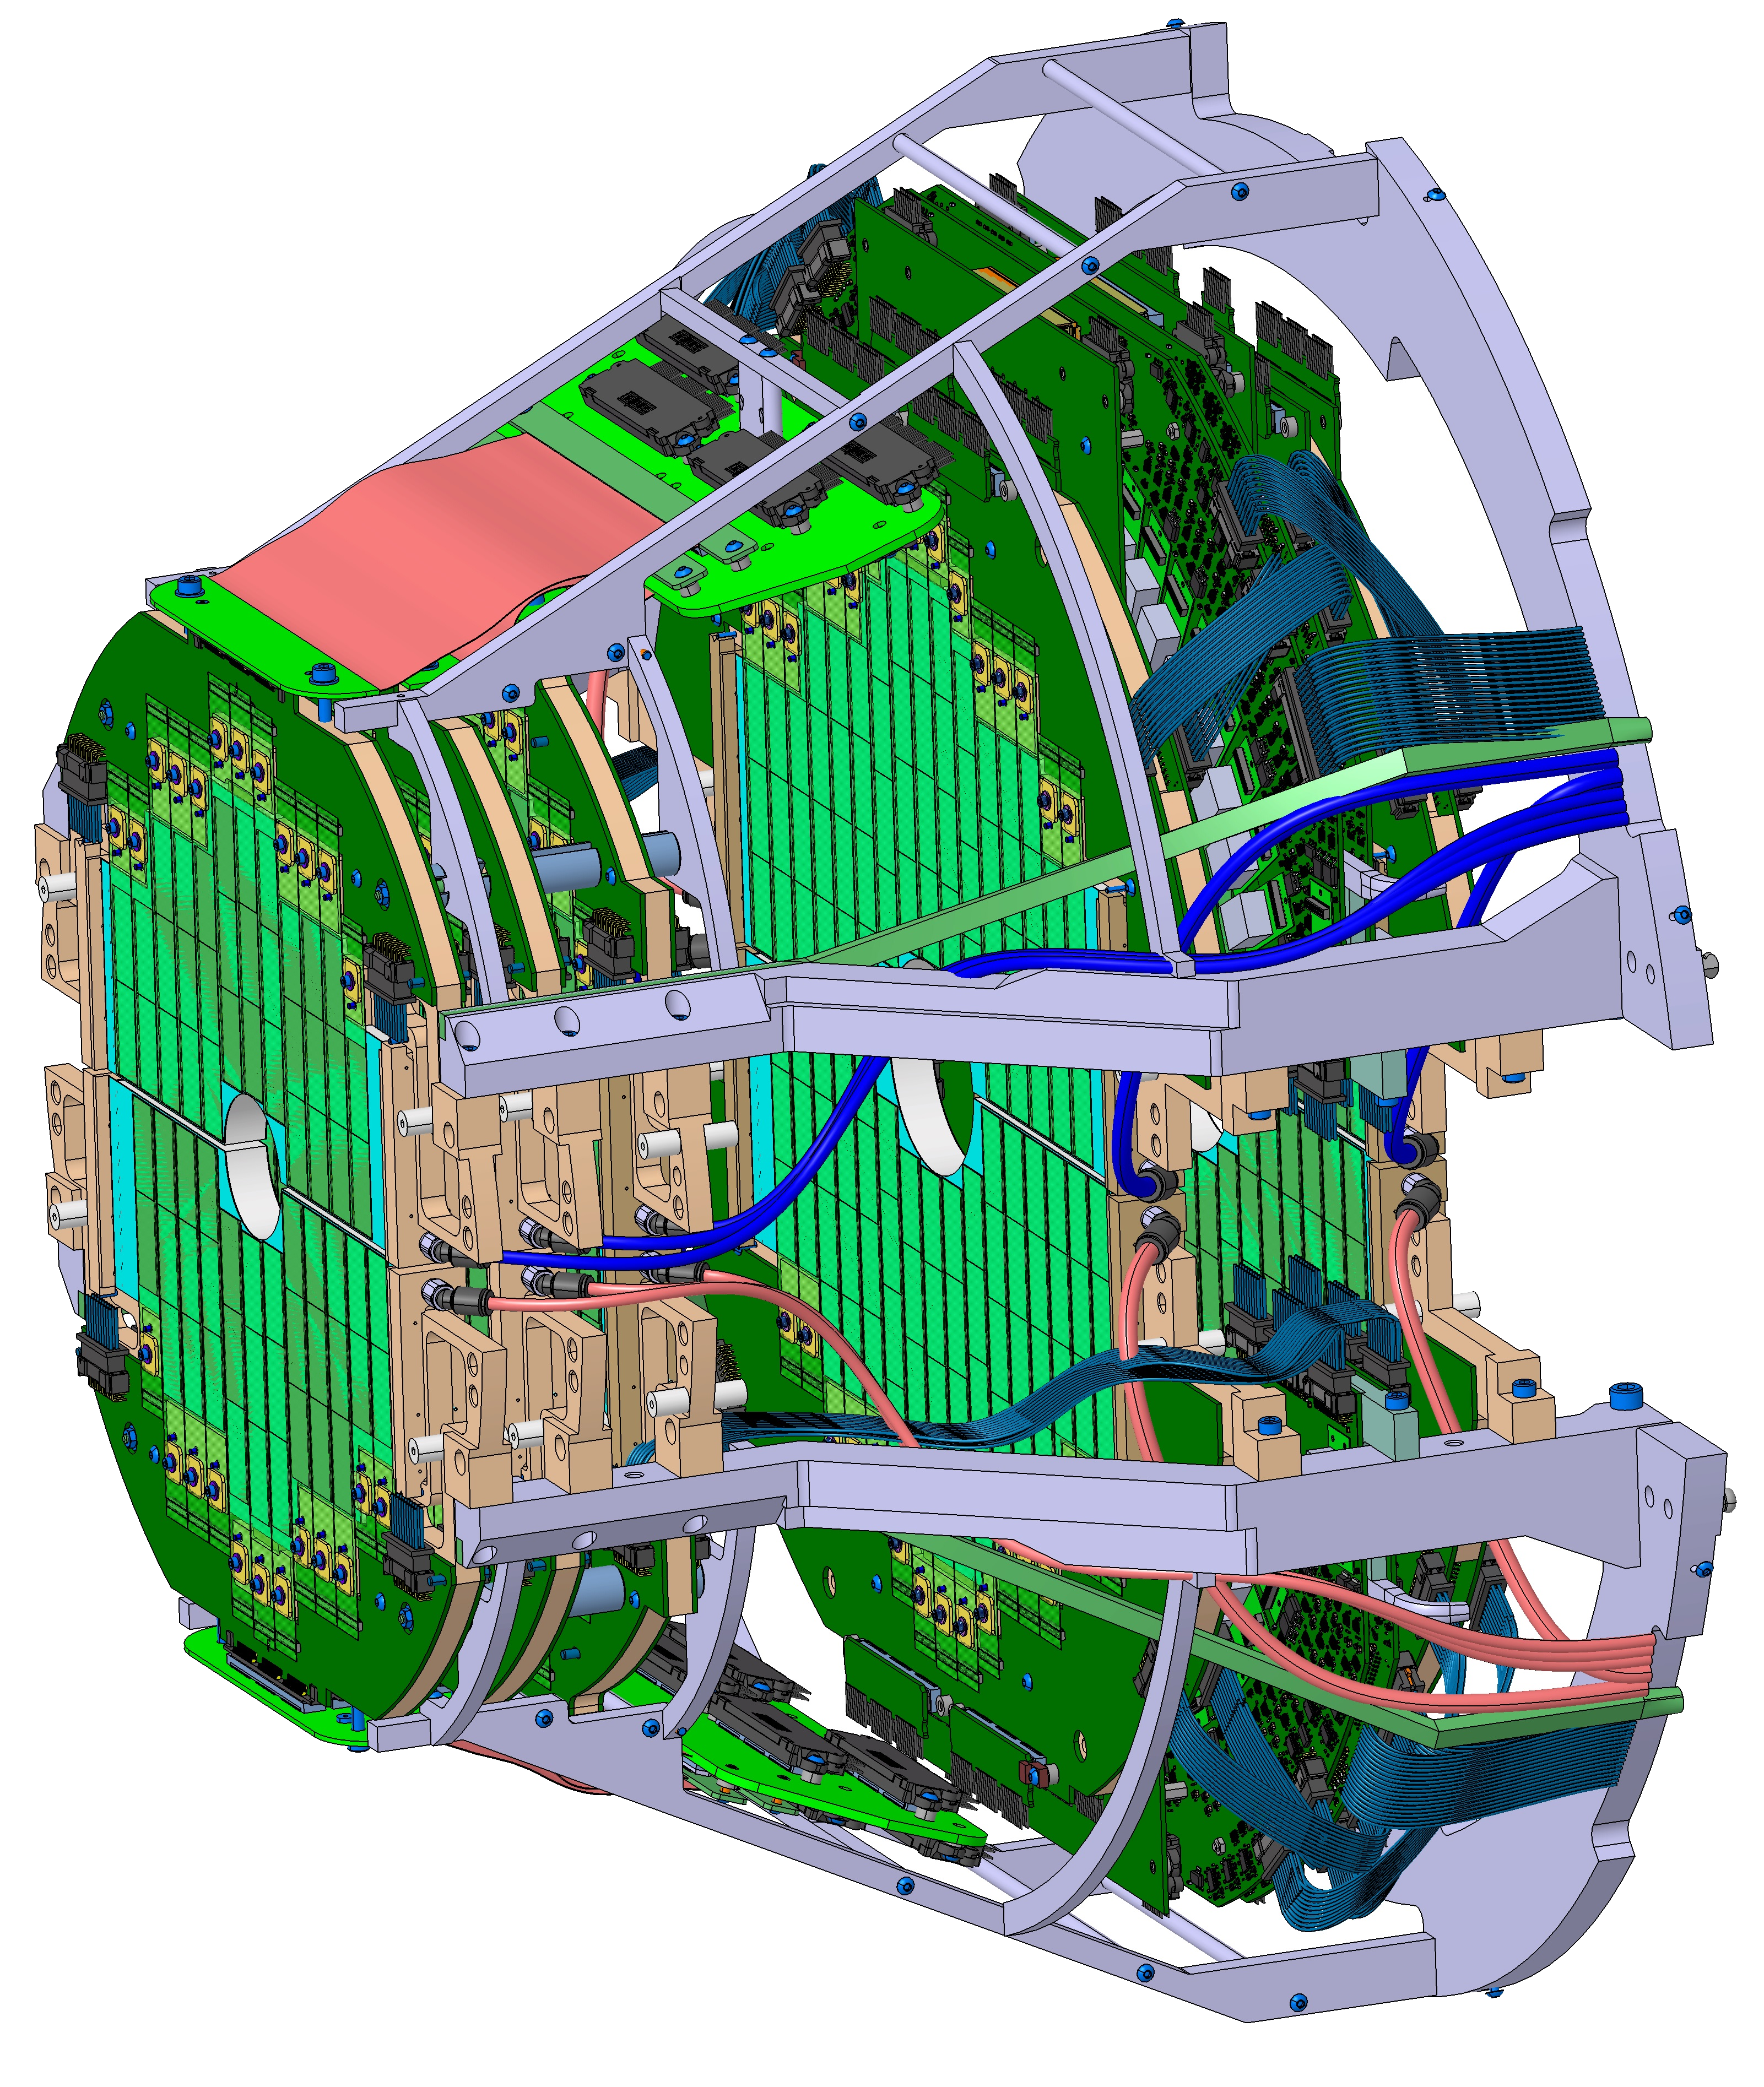
\includegraphics[width=\textwidth]{Figs/MFT_schematic_cropped.png}
                \end{center}
            \end{figure}
        \end{column}
    \end{columns}

\end{frame}

\begin{frame}
    \frametitle{Online-Offline Analysis Framework (O2)}

    \begin{columns}[c]
        \begin{column}{0.5\textwidth}
            \begin{itemize}
                \item Created for Run 3 to deal with untriggered data capture, splitting it into \SI{10}{\milli\second} ``timeframes''
                \item Raw data converted to usable data with ``reconstruction passes''
                \item Then analysed with C\texttt{++} and ROOT for efficient memory and CPU usage
                \item Don't breathe near O2, or it might break
            \end{itemize}
        \end{column}

        \begin{column}{0.5\textwidth}
            \begin{figure}
                \begin{center}
                    \includegraphics[width=\textwidth]{Figs/O2_flow.png}
                \end{center}
            \end{figure}
        \end{column}
    \end{columns}

\end{frame}

\section{Data}

\begin{frame}
    \frametitle{What data are we using?}

    \begin{itemize}
        \item Pilot beam runs 505548 and 505645 from October 2021
        \item Non-nominal centre of mass energy $\sqrt{s}=\SI{900}{\giga\electronvolt}$
        \item Detectors running: ITS, MCH, MFT, MID, TOF, TPC, TRD
    \end{itemize}

\end{frame}

\begin{frame}
    \frametitle{MFT Kinematics (pass3)}

    \begin{columns}[c]
        \begin{column}{0.5\textwidth}
            \begin{figure}
                \begin{center}
                    \includegraphics[width=\textwidth]{Plots/MFT_pass3/eta.png}
                \end{center}
            \end{figure}
            \begin{figure}
                \begin{center}
                    \includegraphics[width=\textwidth]{Plots/MFT_pass3/eta-phi.png}
                \end{center}
            \end{figure}
        \end{column}
        \begin{column}{0.5\textwidth}
            \begin{figure}
                \begin{center}
                    \includegraphics[width=\textwidth]{Plots/MFT_pass3/phi.png}
                \end{center}
            \end{figure}
            \begin{figure}
                \begin{center}
                    \includegraphics[width=\textwidth]{Plots/MFT_pass3/Z_MFT.png}
                \end{center}
            \end{figure}
        \end{column}
    \end{columns}

\end{frame}

\begin{frame}
    \frametitle{MFT x-y plots}

    \begin{columns}[c]
        \begin{column}{0.5\textwidth}
            \begin{figure}
                \begin{center}
                    \includegraphics[width=\textwidth]{Plots/MFT_pass3/x_y_1.png}
                \end{center}
            \end{figure}
            \begin{figure}
                \begin{center}
                    \includegraphics[width=\textwidth]{Plots/MFT_pass3/x_y_3.png}
                \end{center}
            \end{figure}
        \end{column}
        \begin{column}{0.5\textwidth}
            \begin{figure}
                \begin{center}
                    \includegraphics[width=\textwidth]{Plots/MFT_pass3/x_y_2.png}
                \end{center}
            \end{figure}
            \begin{figure}
                \begin{center}
                    \includegraphics[width=\textwidth]{Plots/MFT_pass3/x_y_4.png}
                \end{center}
            \end{figure}
        \end{column}
    \end{columns}

\end{frame}

\begin{frame}
    \frametitle{MFT Kinematics pass3 vs. pass4}

    \begin{columns}[c]
        \begin{column}{0.5\textwidth}
            \begin{figure}
                \begin{center}
                    \includegraphics[width=\textwidth]{Plots/MFT_pass3/eta.png}
                \end{center}
            \end{figure}
            \begin{figure}
                \begin{center}
                    \includegraphics[width=\textwidth]{Plots/MFT_pass3/eta-phi.png}
                \end{center}
            \end{figure}
        \end{column}

        \begin{column}{0.5\textwidth}
            \begin{figure}
                \begin{center}
                    \includegraphics[width=\textwidth]{Plots/MFT_pass4/eta.png}
                \end{center}
            \end{figure}
            \begin{figure}
                \begin{center}
                    \includegraphics[width=\textwidth]{Plots/MFT_pass4/eta-phi.png}
                \end{center}
            \end{figure}
        \end{column}
    \end{columns}

\end{frame}

\begin{frame}
    \frametitle{ITS Kinematics}

    \begin{columns}[c]
        \begin{column}{0.5\textwidth}
            \begin{figure}
                \begin{center}
                    \includegraphics[width=\textwidth]{Plots/ITS/eta.png}
                \end{center}
            \end{figure}
            \begin{figure}
                \begin{center}
                    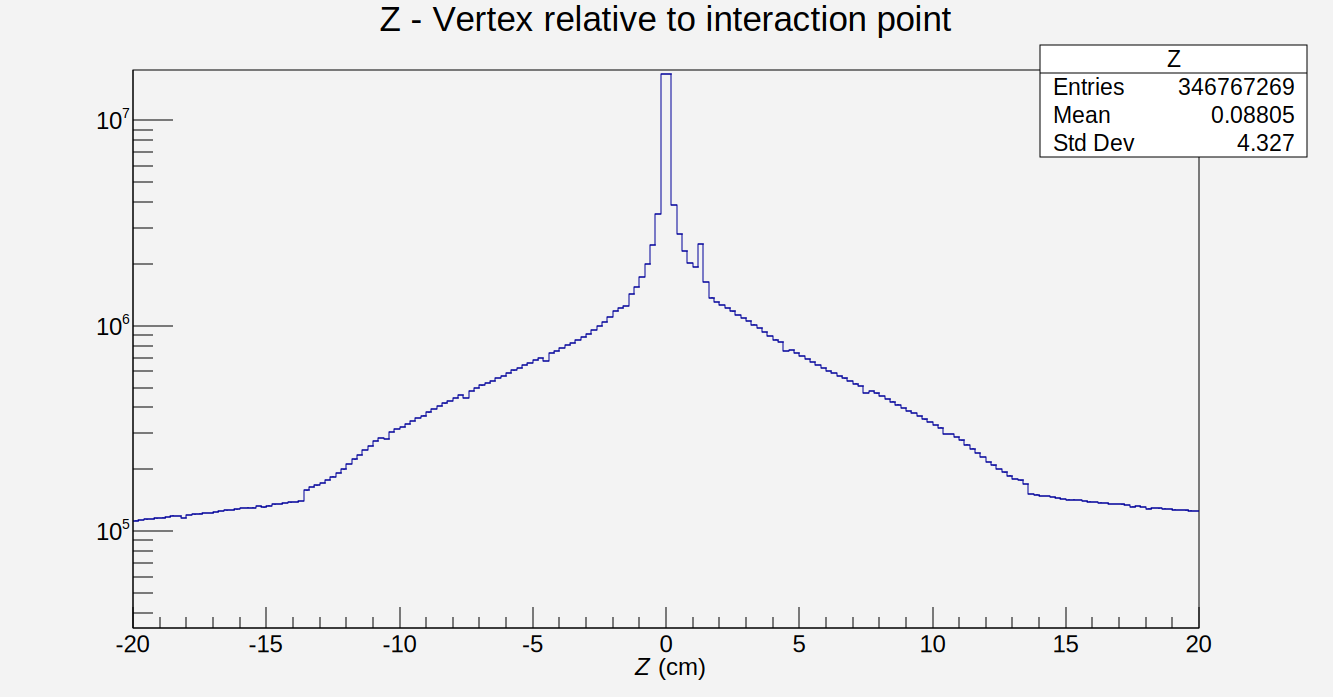
\includegraphics[width=\textwidth]{Plots/ITS/Z.png}
                \end{center}
            \end{figure}
        \end{column}

        \begin{column}{0.5\textwidth}
            \begin{figure}
                \begin{center}
                    \includegraphics[width=\textwidth]{Plots/ITS/phi.png}
                \end{center}
            \end{figure}
            \begin{figure}
                \begin{center}
                    \includegraphics[width=\textwidth]{Plots/ITS/eta-phi.png}
                \end{center}
            \end{figure}
        \end{column}
    \end{columns}

\end{frame}

\section{Conclusion}

\begin{frame}
    \frametitle{Next Steps}

    \begin{itemize}
        \item Why does $Z_{MFT}$ only show the first two disks?
        \item What is different about pass4?
        \item Was ITS working properly/what is that gap in the data?
        \item James mentioned a report but it's probably not that important
    \end{itemize}

\end{frame}

\begin{frame}
    \begin{center}
        {\Huge Thank you!}
    \end{center}

\end{frame}


\end{document}